\documentclass[tikz,border=2pt]{standalone}
\usepackage{pgfplots}
\pgfplotsset{compat=1.7}

\begin{document}
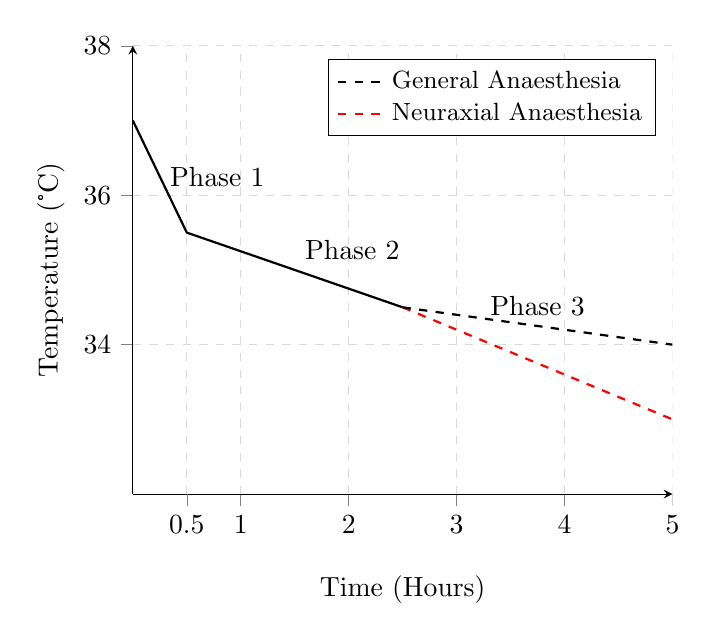
\begin{tikzpicture}


\begin{axis}[
     axis lines=middle,
     grid = major,
     grid style={dashed, gray!30},
	ylabel near ticks,
	xlabel near ticks,
	ymin = 32,
	ymax = 38,
	xmin = 0,
	xmax =5,
	ylabel near ticks,
	xlabel near ticks,
	extra x ticks={0.5},
     xlabel=Time (Hours),
     ylabel=Temperature (°C),
     tick align=outside,
	legend pos= north east,
	legend style={font=\small, cells={align=left}},
legend cell align={left}]

\draw[black, thick] (axis cs: 0, 37) -- node[right]{Phase 1} (axis cs: 0.5, 35.5) -- node[above right]{Phase 2}(axis cs: 2.5, 34.5);
\draw[red, thick, dashed] (axis cs: 2.5, 34.5) -- (axis cs: 5, 33);
\draw[black, thick, dashed] (axis cs: 2.5, 34.5) -- node[above]{Phase 3} (axis cs: 5, 34);

\addlegendimage{black, thick, dashed};
\addlegendentry{General Anaesthesia};
\addlegendimage{red, thick, dashed};
\addlegendentry{Neuraxial Anaesthesia};

\end{axis}

\end{tikzpicture} 
\end{document}